\section{The PID actions}
\subsection{}

\begin{frame}
\frametitleTC{Foreword}
\framesubtitleTC{}
\myPause
 \begin{itemize}[<+-| alert@+>]
 \item We carry out this treatise in a DT LTI (comments on saturations later on) with sampling time $T_s$.
 \item This said, from the PID quasi-algorithm on slide~\ref{pag:PID-quasi-alg} we get the error-to-action
       transfer functions
       \begin{displaymath}
        \begin{array}{lclcl}
         C_P(z) &:=& \cfrac{u_P(k)}{e(k)} &=& K, \\ \\
         C_I(z) &:=& \cfrac{u_I(k)}{e(k)} &=& \cfrac{KT_s}{T_i} \, \cfrac{z}{z-1}, \\ \\
         C_D(z) &:=& \cfrac{u_D(k)}{e(k)} &=& \cfrac{KT_d(1-\beta)}{T_s} \, \cfrac{z-1}{z-\beta}.
        \end{array}
       \end{displaymath}
 \end{itemize}
\end{frame}

\begin{frame}
\frametitleTC{Foreword}
\framesubtitleTC{}
\myPause
 \begin{itemize}[<+-| alert@+>]
 \item Block diagram of a PID control loop evidencing the three actions
       \begin{center}
        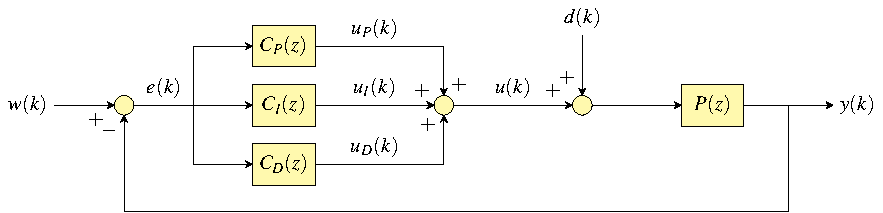
\includegraphics[width=0.85\columnwidth]{./Unit-07/img/PIDloop-actions.pdf}
       \end{center}
 \item \vspace{2mm}NOTE: the disturbance is added to the control signal, i.e., $H(z)=P(z)$;\\
       such a disturbance is called a \TC{load} or a \TC{matched} disturbance.
 \item Load disturbances can arise every time the disturbing and the\\
       control actions are physically homogeneous, which is not infrequent\\
       ---e.g., the control is allocating a resource, and the disturbing entity\\
       is somebody subtracting some amount of the same resource.
 \end{itemize}
\end{frame}

\begin{frame}
\frametitleTC{Computing the three actions}
\framesubtitleTC{}
\myPause
 \begin{itemize}[<+-| alert@+>]
 \item From
       \begin{center}
        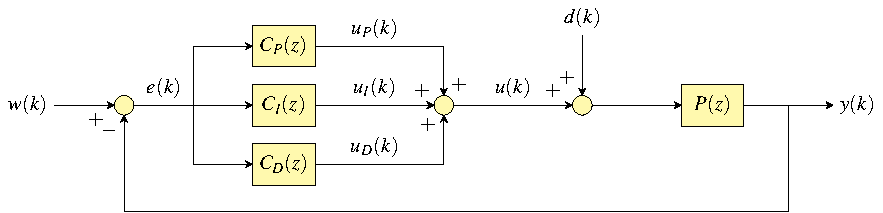
\includegraphics[width=0.70\columnwidth]{./Unit-07/img/PIDloop-actions.pdf}
       \end{center}
       and setting $C(z) = C_P(z)+C_I(z)+C_D(z)$, we readily get
       \begin{displaymath}
        \begin{array}{llcll}
          \cfrac{u_P(k)}{w(k)} &\mkern-12mu =  \cfrac{C_P(z)}{1+P(z)C(z)},       &\quad&
          \cfrac{u_P(k)}{d(k)} &\mkern-12mu = -\cfrac{P(z)C_P(z)}{1+P(z)C(z)}, \\
          \cfrac{u_I(k)}{w(k)} &\mkern-12mu =  \cfrac{C_I(z)}{1+P(z)C(z)},       &\quad&
          \cfrac{u_I(k)}{d(k)} &\mkern-12mu = -\cfrac{P(z)C_I(z)}{1+P(z)C(z)}, \\
          \cfrac{u_D(k)}{w(k)} &\mkern-12mu =  \cfrac{C_D(z)}{1+P(z)C(z)},       &\quad&
          \cfrac{u_D(k)}{d(k)} &\mkern-12mu = -\cfrac{P(z)C_D(z)}{1+P(z)C(z)}.
        \end{array}
       \end{displaymath}
 \end{itemize}
\end{frame}

\begin{frame}
\frametitleTC{Computing the three actions}
\framesubtitleTC{}
\myPause
 \begin{itemize}[<+-| alert@+>]
 \item We now examine the behaviour of the scheme above with a first-order process\\
       with gain $\mu$ and time constant $T$, that recalling slide~\ref{pag:FOsystem-DT}, in transfer function\\
       form reads
       \begin{displaymath}
        P(z) = \frac{\mu\frac{T_s}{T+T_s}z}{z-\frac{T}{T+T_s}}.
       \end{displaymath}
 \item We start out with a PI tuned by cancellation as per the formul{\ae} of slide~\ref{pag:PItuning-lambda},\\
       that is,
       \begin{displaymath}
        K   = \frac{T}{\lambda\mu}, \quad
        T_i = T.
       \end{displaymath}
       where $\lambda$ is the desired closed-loop time constant (1/5 of the desired\\
       settling time).
 \item Then we add a bit of D action, and comment on all of the results.
 \end{itemize}
\end{frame}

\begin{frame}[fragile]
\frametitleTC{Computing the three actions}
\framesubtitleTC{Scilab script (1/3)}
\myPause
 {\scriptsize
 \begin{verbatim}
 clear; clc;                                          // clear workspace & console
 z      = %z;                                         // allow to omit lots of %'s below

 mu     = 1;                                          // process gain  
 T      = 10;                                         // and time constant
 lambda = 4;                                          // desired closed-loop TC
 Beta   = 0.6;                                        // derivative filter
 Ts     = 1;                                          // sampling time
 tfin   = 50;                                         // simulation end time

 K      = T/lambda/mu;                                // PID tuning
 Ti     = T;
 Td     = 0;

 P      = syslin(Ts,z*Ts/(T+Ts)/(z-T/(T+Ts)));        // process and controller
 Cp     = K;                                          // transfer functions:
 Ci     = syslin(Ts,K*Ts/Ti*z/(z-1));                 // a number instead of
 Cd     = syslin(Ts,K*Td*(1-Beta)/Ts*(z-1)/(z-Beta)); // 'd' sets the sampling
 C      = Cp+Ci+Cd;                                   // time for a DT system
 \end{verbatim}
 }
\end{frame}

\begin{frame}[fragile]
\frametitleTC{Computing the three actions}
\framesubtitleTC{Scilab script (2/3)}
\myPause
 {\scriptsize
 \begin{verbatim}
 w2y    = tf2ss(C*P/(1+C*P));           // transfer function from w to y
 d2y    = tf2ss(P/(1+C*P));             // transfer function from d to y
 w2u    = tf2ss(C/(1+C*P));             // transfer function from w to u
 d2u    = tf2ss(-C*P/(1+C*P));          // transfer function from d to u
 w2up   = tf2ss(Cp/(1+C*P));            // transfer function from w to up
 w2ui   = tf2ss(Ci/(1+C*P));            // transfer function from w to ui
 w2ud   = tf2ss(Cd/(1+C*P));            // transfer function from w to ud
 d2up   = tf2ss(-P*Cp/(1+C*P));         // transfer function from d to up
 d2ui   = tf2ss(-P*Ci/(1+C*P));         // transfer function from d to ui
 d2ud   = tf2ss(-P*Cd/(1+C*P));         // transfer function from d to ud

 t      = 0:Ts:tfin;                    // time vector
 wd     = ones(t);                      // step with one zero sample 
 wd(1)  = 0;                            // at the beginning
 yw     = dsimul(w2y,wd)';              // y in response to a w step
 yd     = dsimul(d2y,wd)';              // y in response to a d step
 uw     = dsimul(w2u,wd)';              // u in response to a w step
 ud     = dsimul(d2u,wd)';              // u in response to a d step
 upidw  = dsimul([w2up;w2ui;w2ud],wd)'; // u{p,i,d} in response to a w step
 upidd  = dsimul([d2up;d2ui;d2ud],wd)'; // u{p,i,d} in response to a d step
 \end{verbatim}
 }
\end{frame}

\begin{frame}[fragile]
\frametitleTC{Computing the three actions}
\framesubtitleTC{Scilab script (3/3)}
\myPause
 {\scriptsize
 \begin{verbatim}
 hf=scf(0); clf; hf.figure_size = [1200,700];                    // plot stuff: see the Scilab
 subplot(321); title('Responses to a w unit step'); ylabel('y'); // documentation for technical
   plot(0,0,'k');                                                // details here inessential
   plot(t',ones(t'),'k:');
   plot(t',yw,'b','linewidth',4);
 subplot(322); title('Responses to a d unit step'); 
   plot(t',zeros(t'),'k:');
   plot(t',yd,'b','linewidth',4);
 subplot(323); xlabel('time'); ylabel('u,up,ui,ud (g,b,r,m)');
   plot(0,0,'k');
   plot(t',uw,'g','linewidth',4);
   plot(t',upidw(:,1),'b','linewidth',2);
   plot(t',upidw(:,2),'r','linewidth',2);
   plot(t',upidw(:,3),'m','linewidth',2);
 subplot(324); xlabel('time');
   plot(0,0,'k');
   plot(t',ud,'g','linewidth',4);
   plot(t',upidd(:,1),'b','linewidth',2);
   plot(t',upidd(:,2),'r','linewidth',2);
   plot(t',upidd(:,3),'m','linewidth',2);
 \end{verbatim}
 }
\end{frame}

\begin{frame}
\frametitleTC{Observing the three actions}
\framesubtitleTC{Scilab script -- example of the output}
\myPause
 \begin{center}
  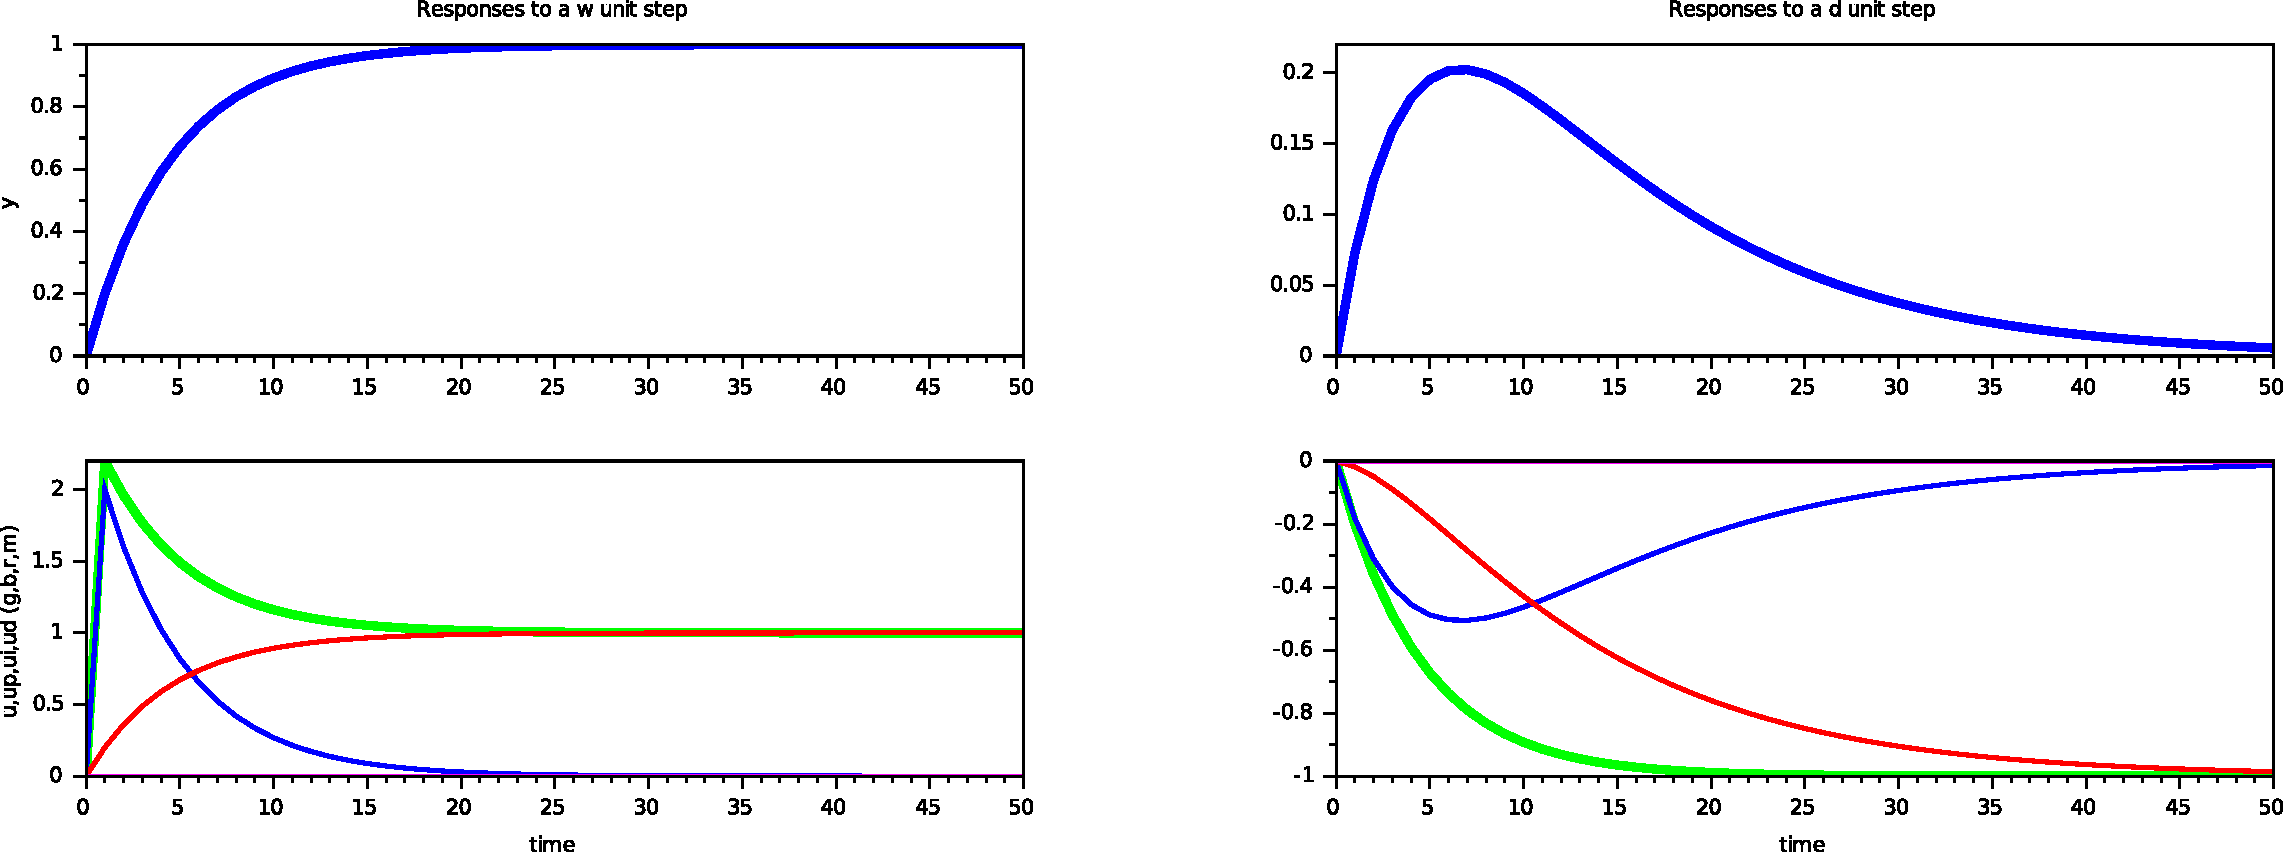
\includegraphics[width=0.75\columnwidth]{./Unit-07/img/PIDactions-scilab-01.pdf}
 \end{center}
 \begin{itemize}[<+-| alert@+>]
 \item Top row: responses of $y$ to a unit step on $w$ (left) and on $d$ (right).
 \item Bottom row: breakdown of $u$ (green) into $u_P$ (blue), $u_I$ (red),\\
       and $u_D$ (magenta).
 \item Note that at steady state $u$ is made only of integral action.
 \item Let us now play around with PID parameters, also not following the\\
       tuning rule exactly, and see what happens.
 \end{itemize}
\end{frame}

\begin{frame}[fragile]
\frametitleTC{Observing the three actions}
\framesubtitleTC{Playing around with PID parameters -- a few suggestions (1/3)}
\myPause
 \begin{itemize}[<+-| alert@+>]
 \item Add some D action:
       {\scriptsize
       \begin{verbatim}
       K   = T/lambda/mu;
       Ti  = T;
       Td  = 0.2*Ti;
       \end{verbatim}
       }
 \item \vspace{-3mm}Speeds up initial transient, hardly any effect on settling time, just a \emph{very} small\\
       overshoot:
       \begin{center}
        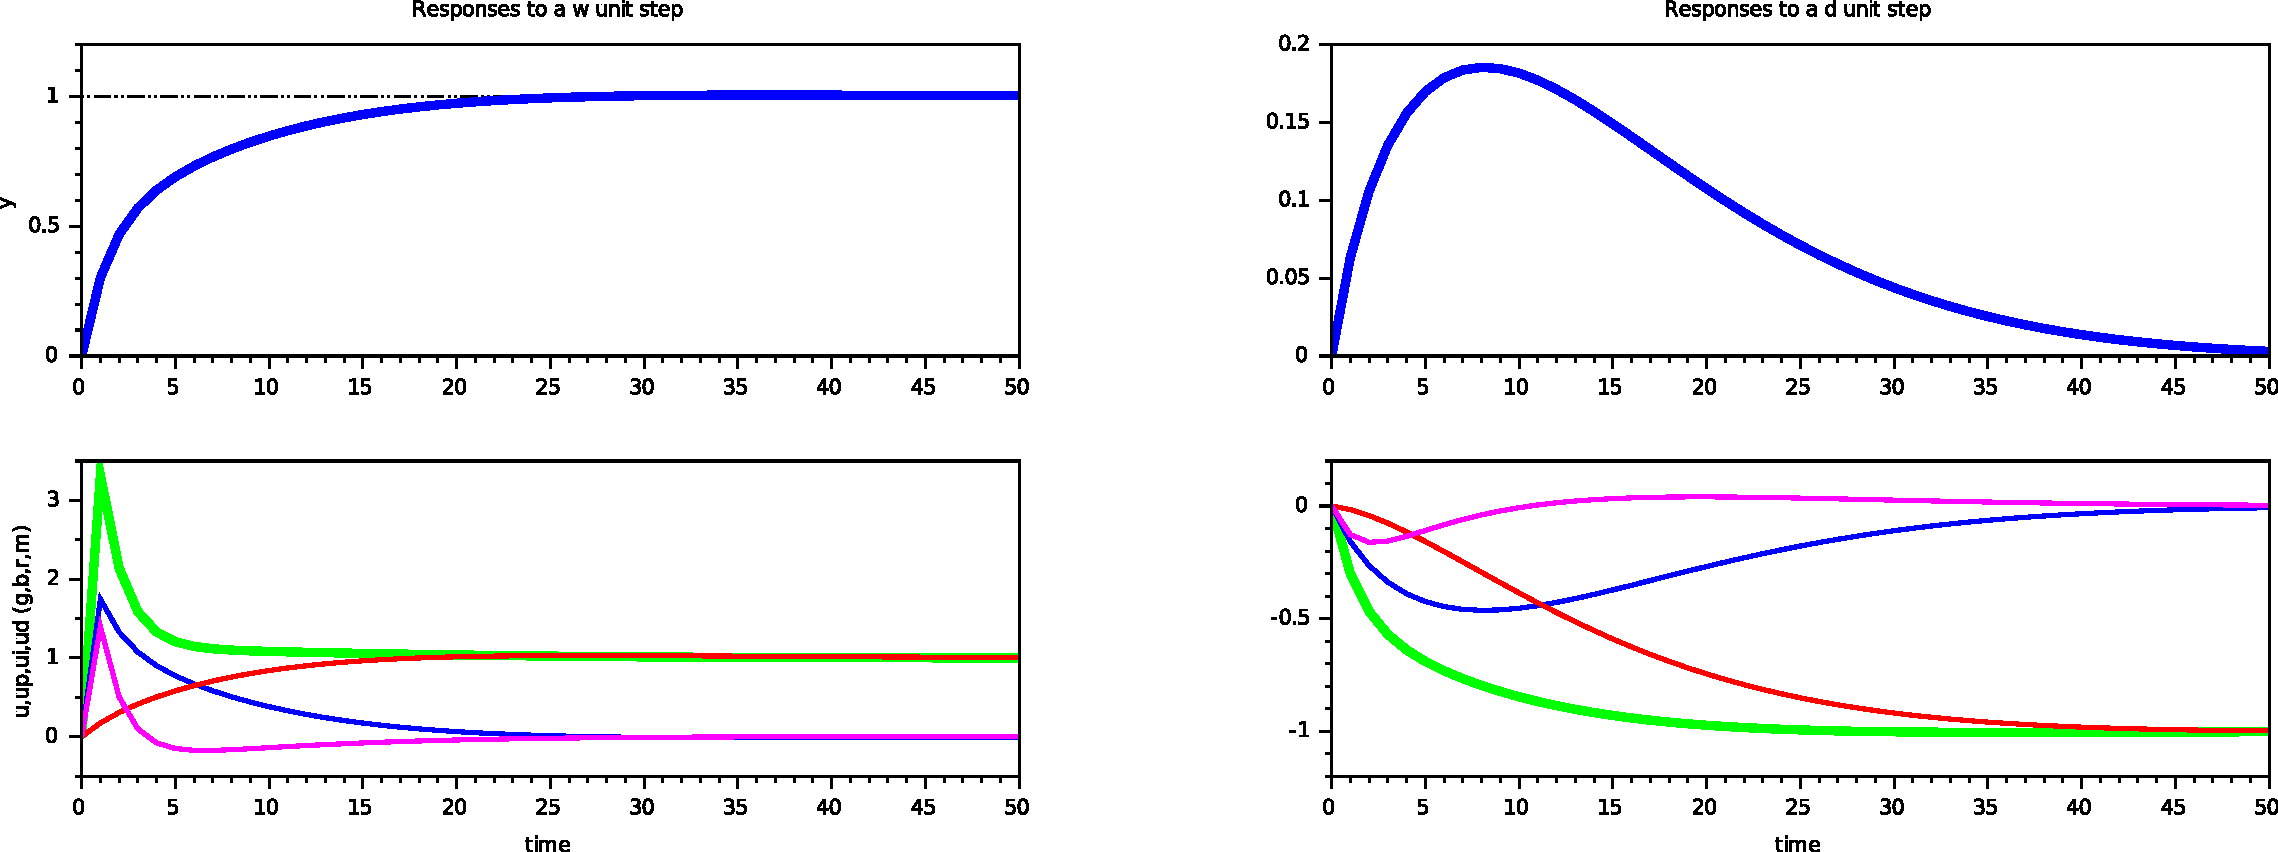
\includegraphics[width=0.60\columnwidth]{./Unit-07/img/PIDactions-scilab-02.pdf}
       \end{center}
 \item Note that clearly the D action vanishes as well toward steady state \\
       (and faster than P). 
 \end{itemize}
\end{frame}

\begin{frame}[fragile]
\frametitleTC{Observing the three actions}
\framesubtitleTC{Playing around with PID parameters -- a few suggestions (2/3)}
\myPause
 \begin{itemize}[<+-| alert@+>]
 \item Back to PI, but halve the integral time:
       {\scriptsize
       \begin{verbatim}
       K   = T/lambda/mu;
       Ti  = 0.5*T;
       Td  = 0;
       \end{verbatim}
       }
 \item \vspace{-3mm}Disturbance response improved at the cost of a slight oscillation\\
       ---i.e., some stability reduction:
       \begin{center}
        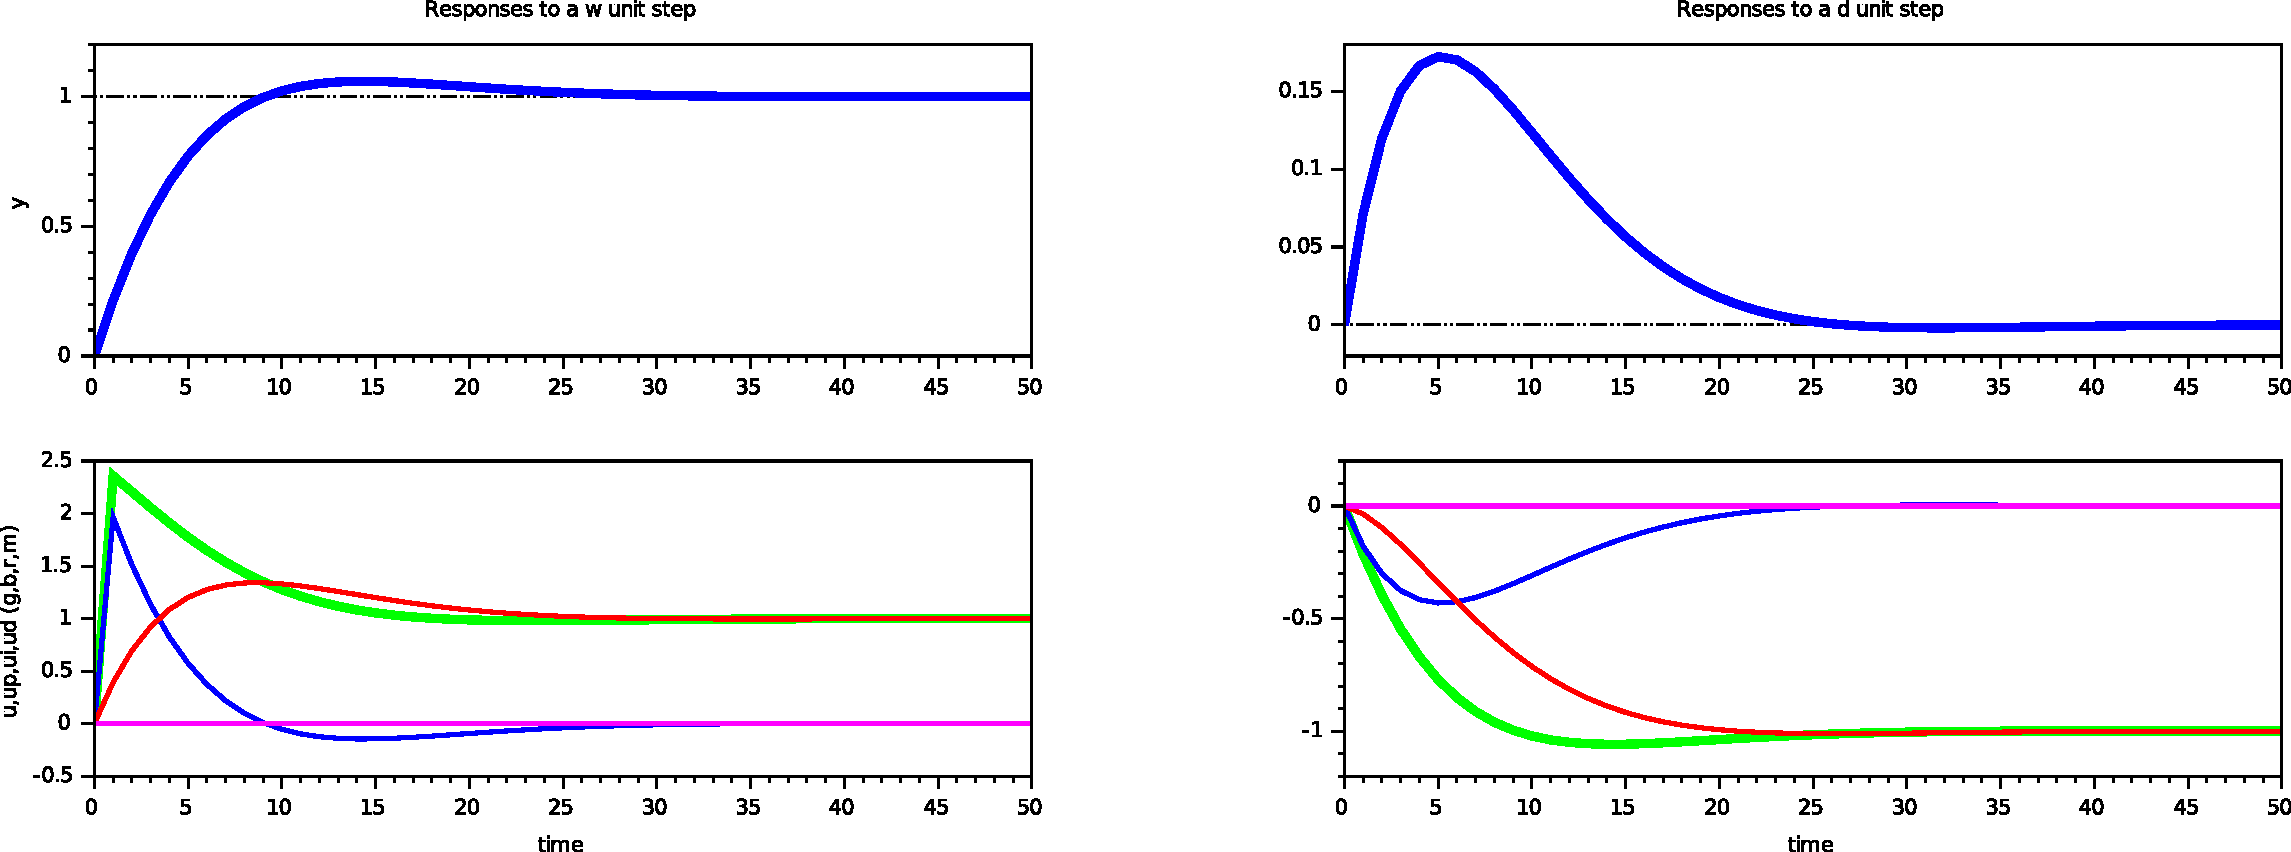
\includegraphics[width=0.60\columnwidth]{./Unit-07/img/PIDactions-scilab-03.pdf}
       \end{center}
 \item Try adjusting $K$ to eliminate the oscillation in the set point response.\\
       Do you succeed? Or just alter the oscillation period?
 \end{itemize}
\end{frame}

\begin{frame}[fragile]
\frametitleTC{Observing the three actions}
\framesubtitleTC{Playing around with PID parameters -- a few suggestions (3/3)}
\myPause
 \begin{itemize}[<+-| alert@+>]
 \item PID again, but with a definitely excessive integral time:
       {\scriptsize
       \begin{verbatim}
       K   = T/lambda/mu;
       Ti  = 4*T;
       Td  = 0.2*Ti;
       \end{verbatim}
       }
 \item \vspace{-3mm}When P and D vanish, I is still far from playing its full role:
       \begin{center}
        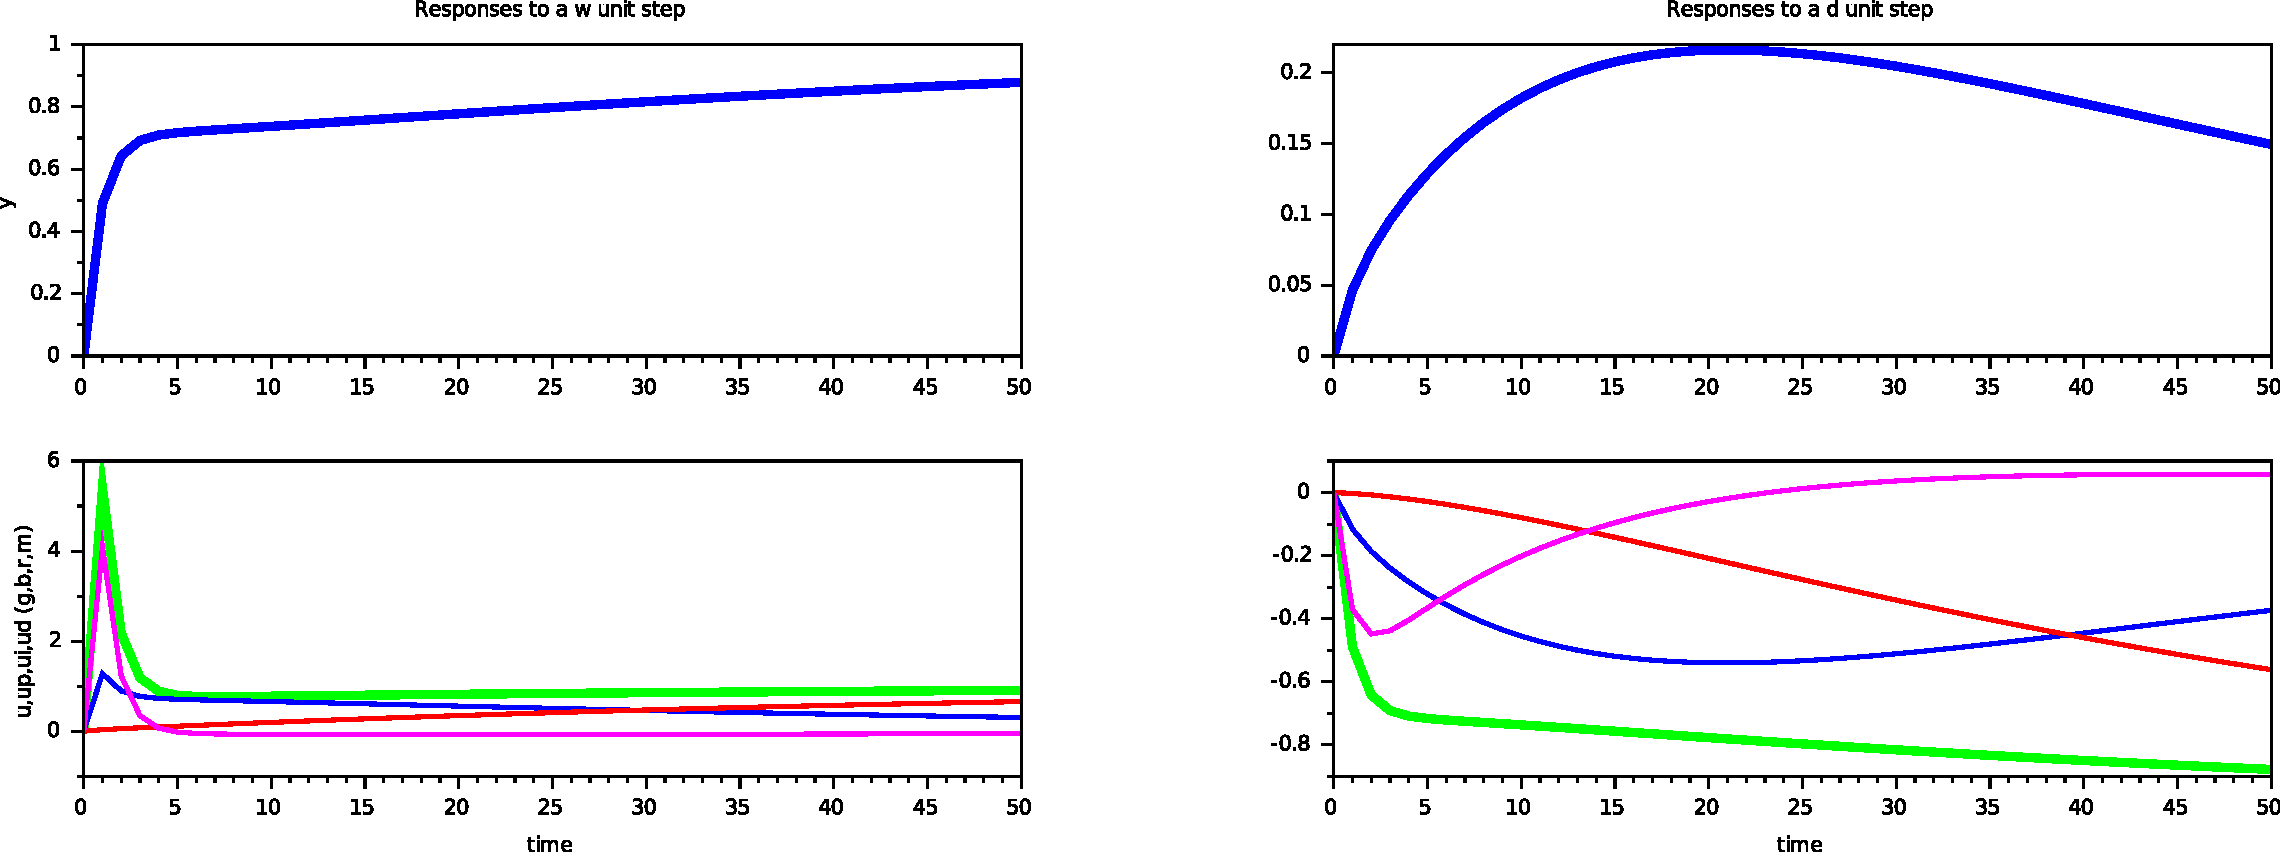
\includegraphics[width=0.60\columnwidth]{./Unit-07/img/PIDactions-scilab-04.pdf}
       \end{center}
 \item Try removing the D action. What effects do you observe on the set\\ 
       point and the disturbance response? Do these correspond to your\\
       expectations?
 \end{itemize}
\end{frame}

\begin{frame}[fragile]
\frametitleTC{The P, I, and D actions}
\framesubtitleTC{Suggestions for further activities}
\myPause
 \begin{itemize}[<+-| alert@+>]
 \item Take the Scilab script above and add some noise on the feedback path---i.e., the \TC{measurement}
       of $y$ fed back to $C$ is corrupted by noise. Hint: Scilab has a \texttt{rand()} and a \texttt{randn()}
       function for uniformly and normally distributed random numbers.
 \item Always remember:
       \begin{itemize}[<+-| alert@+>]
       \item we would like to control physical quantities,
       \item but we can only control measurements.
       \end{itemize}
 \item \vfill Experiment with different numbers, observe, and comment.
 \end{itemize}
\end{frame}

\begin{frame}[fragile]
\frametitleTC{The P, I, and D actions}
\framesubtitleTC{Takeaways}
\myPause
 \begin{itemize}[<+-| alert@+>]
 \item Looking at a response and diagnosing: too much P action, too few I,...
 \item A keyword for the curious here is ``tuning maps''.
 \item \vspace{2mm} Use your \TC{systems theory} knowledge to confirm or debunk some common beliefs:
       \begin{itemize}[<+-| alert@+>]
       \item adding D always makes a system faster --- sure, given one of the tests above?
       \item too much D destabilises --- hmmm, or maybe just amplifies noise?
       \item increasing $K$ does not reject disturbances faster, for that you need\\
             to reduce $T_i$ --- i.e., not just tune by cancellation,
       \item ...and so forth.
       \end{itemize}
 \item If interested go through the many PID-related web sites, read, test\\
       (you have \TC{methods} \& tools) and subject the material you found\\
       to a system-theoretically educated analysis.
 \item This is what we meant right from the outset for ``using (PID)\\
       control consciously''. 
 \end{itemize}
\end{frame}

%Myths debunked
% D makes faster...

%Lessons learnt:
% diagnose, tuning maps

